\chapter{Experimentación y Resultados}
    Aquí se presentaran los resultados del \textbf{Análisis a Priori y Posteriori} de cada algoritmo solicitado respectivamente.
    
\section{Algoritmo 1: Fibonacci Iterativo}
    El algoritmo codificado en \textit{Python} fue testeado en un entorno virtual de Linux, donde el algoritmo pudo calcular al menos 900 elementos de la serie de Fibonacci.
    \subsection{Analisis a Priori }
        La figura \ref{fig:iterativo_f} presenta el análisis a priori realizado sobre el código fuente del algoritmo de la sucesión de Fibonacci recursiva. Concluyendo que el algoritmo presenta una complejidad lineal \(f(n) = O(n)\) porque en cada iteración solamente se asignan dos variables y se realiza una suma.
        
        \begin{figure}[htp!]
            \centering
            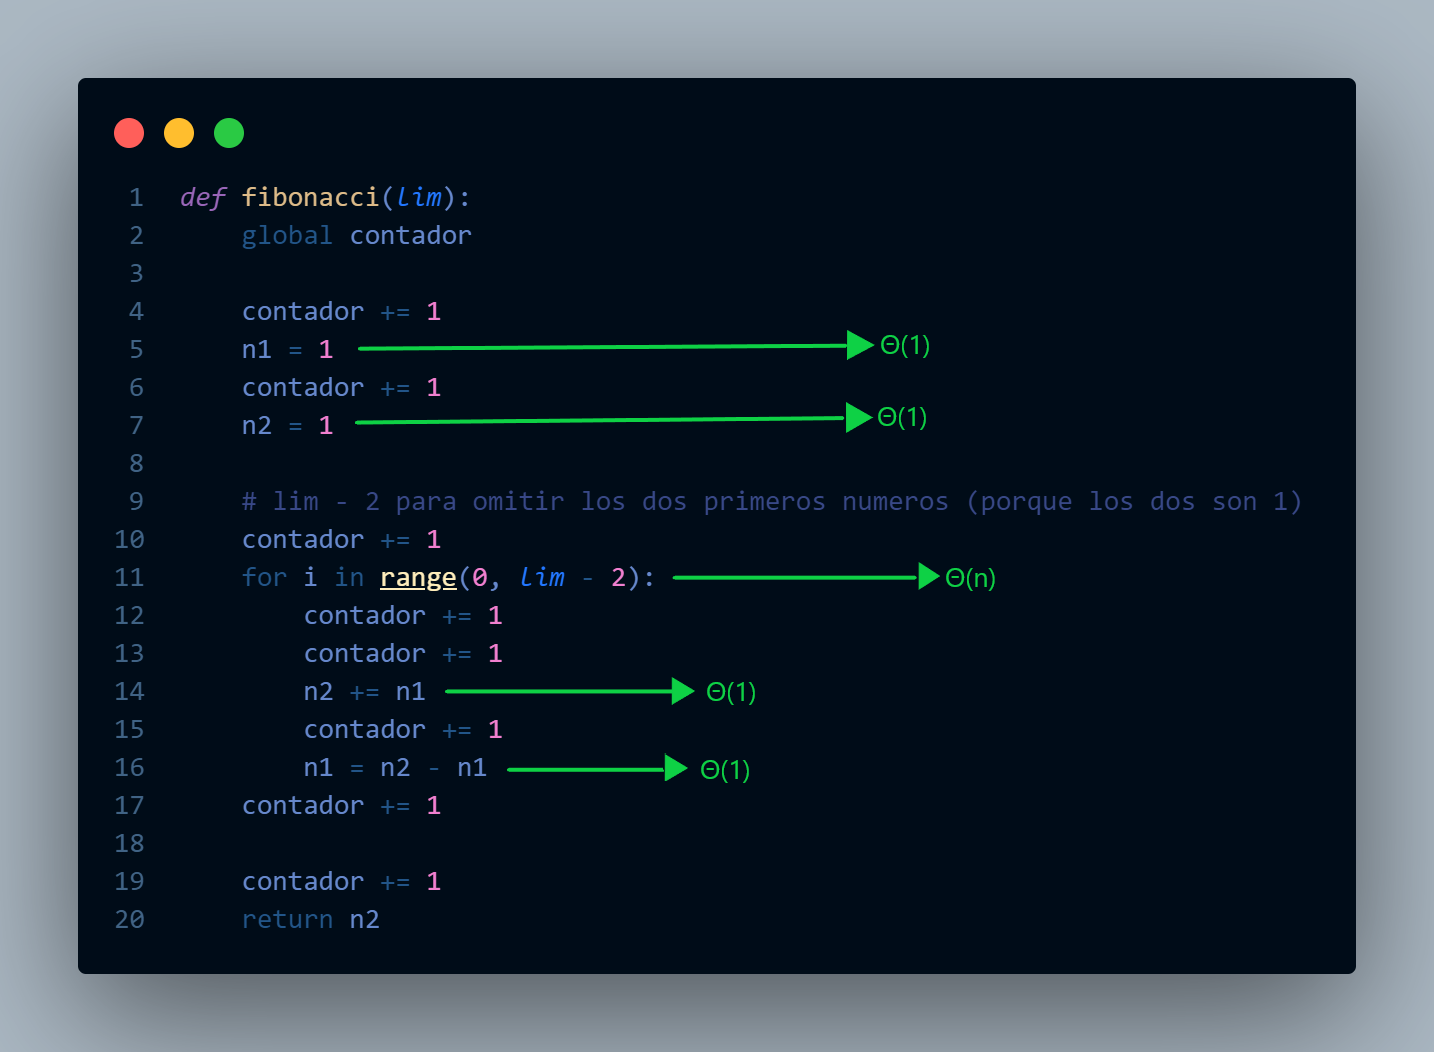
\includegraphics[width=0.7 \textwidth]{Images/priori_iterativo.png}
            \caption{Analisis a Priori: Fibonacci Iterativo}
            \label{fig:iterativo_f}
        \end{figure}
    
    \newpage    
    \subsection{Analisis a Posteriori}
        En el análisis posteriori se verifica el análisis a priori, efectivamente es una función lineal que incrementa en tiempo como se vayan sumando más entradas. Para la gráfica mostrada a continuación (figura \ref{fig:iterativo2_f}) se muestran pocos elementos para notar el crecimiento en la función.
        \begin{figure}[htp!]
            \centering
            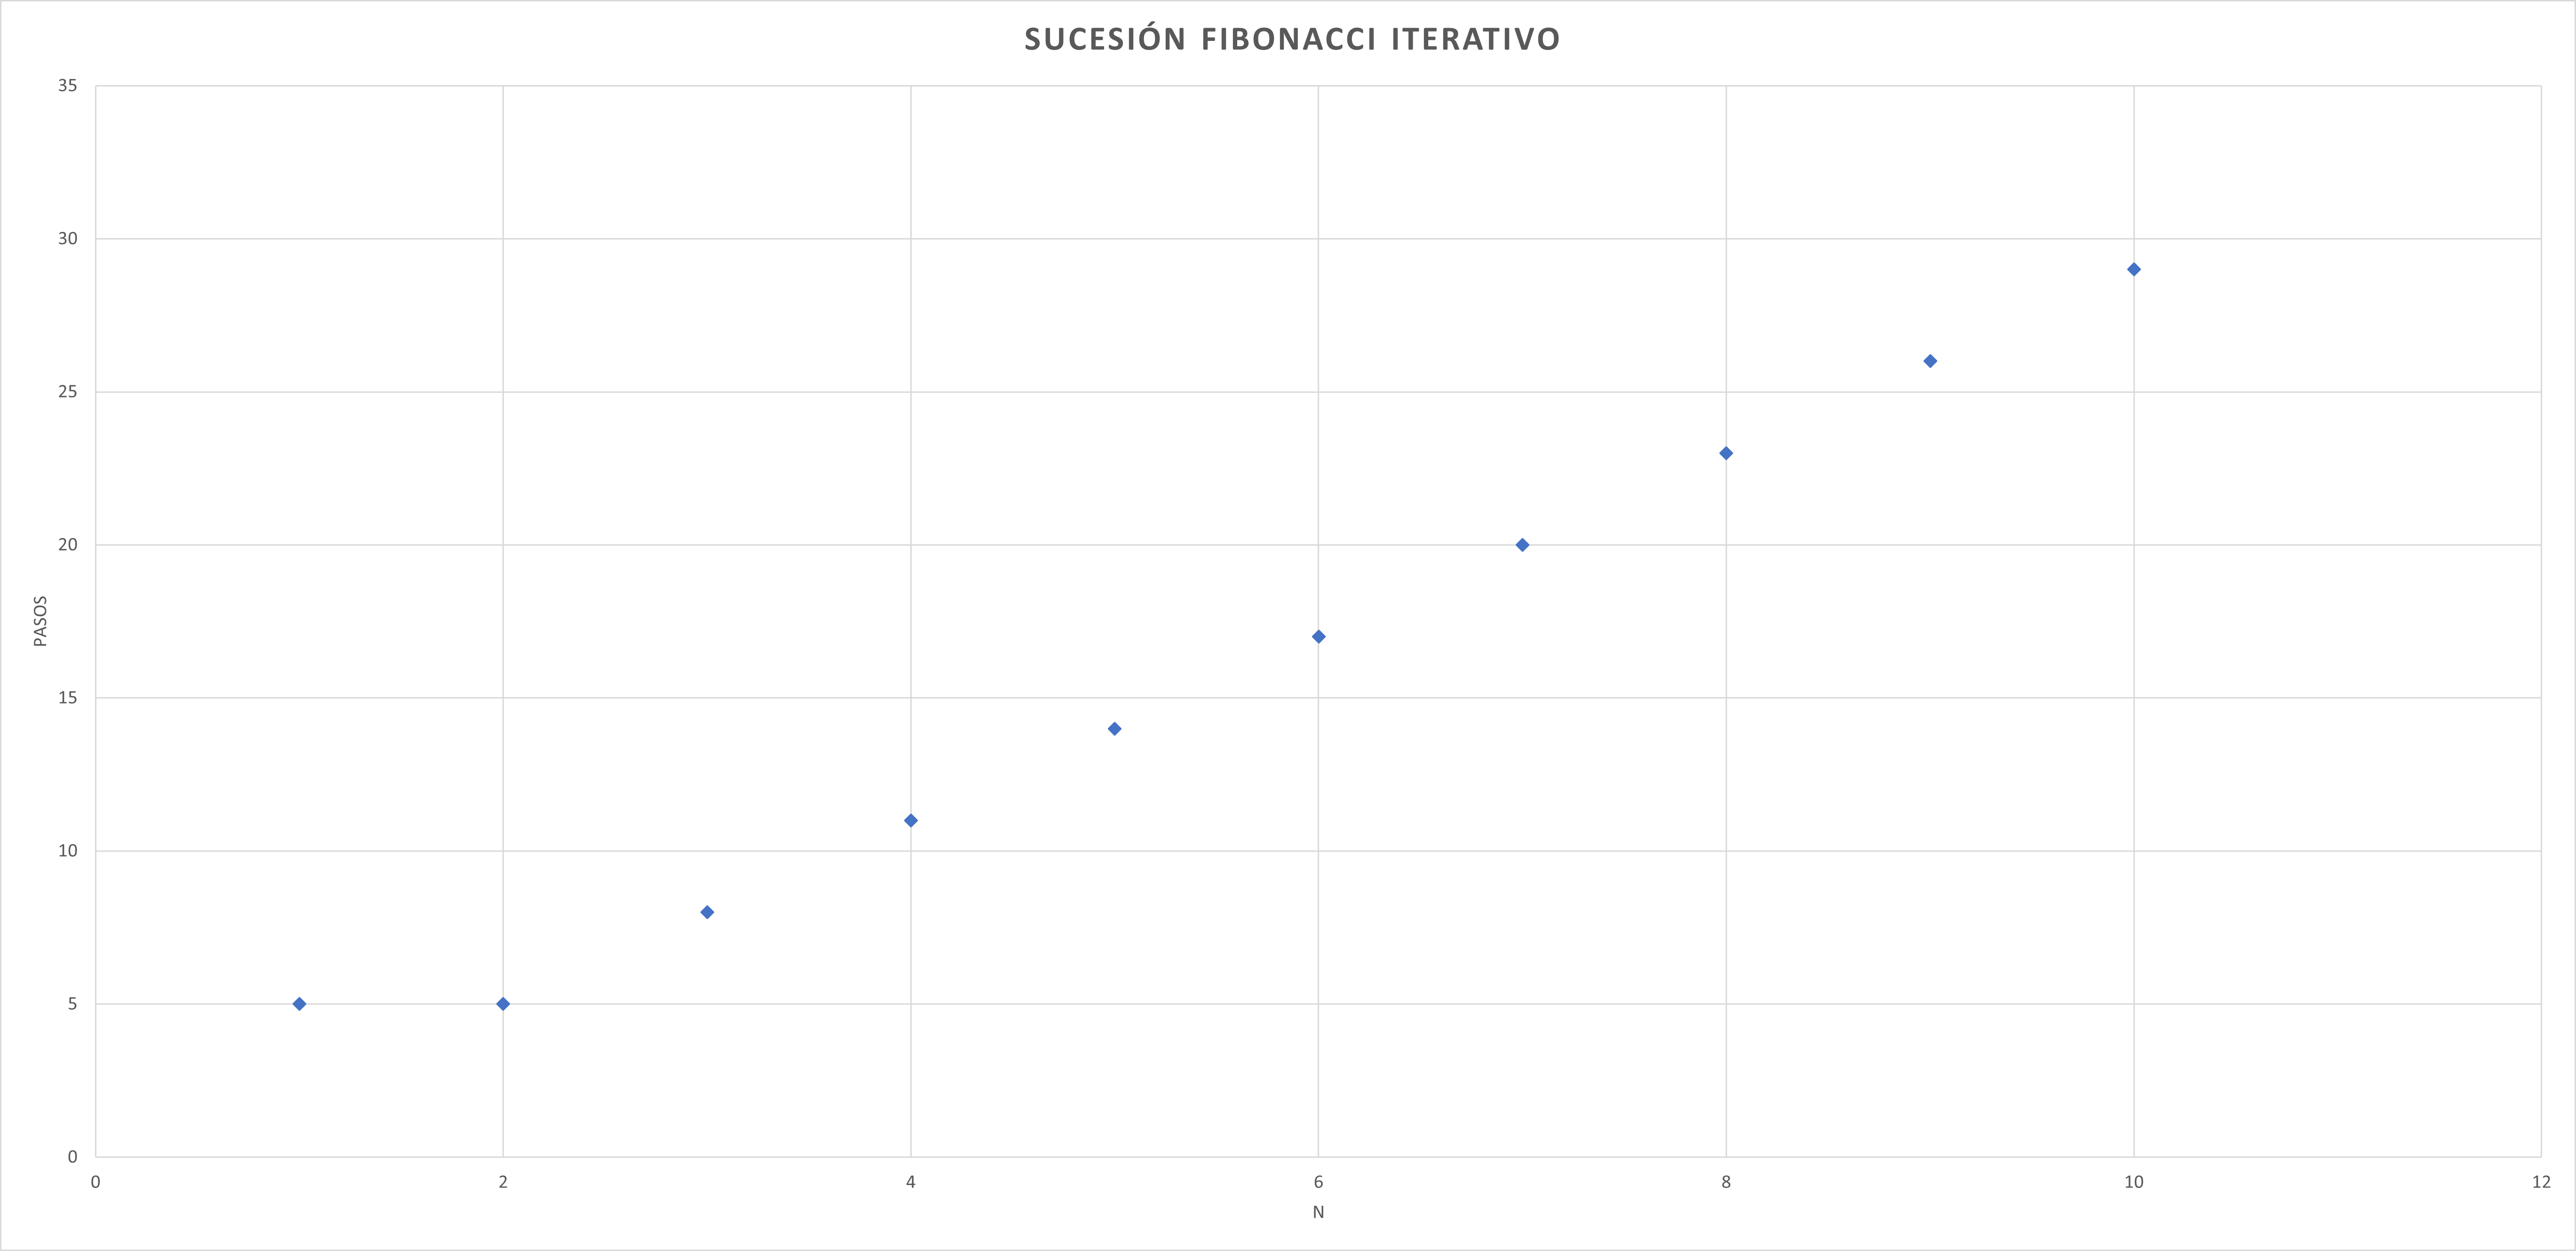
\includegraphics[width=1 \textwidth]{Images/posteriori_iterativo.png}  
            \caption{Analisis a Posteriori: Fibonacci Iterativo}
            \label{fig:iterativo2_f}
        \end{figure}
    
    
    
    
    \newpage
    \section{Algoritmo 2: Fibonacci Recursivo}
        El algoritmo codificado en \textit{Python} fue testeado en un entorno virtual de Linux, donde el algoritmo pudo calcular al menos 900 elementos de la serie de Fibonacci con un tiempo de ejecución creciente. 
    \subsection{Analisis a Posteriori}
        El algoritmo analizado en posteriori, dio como resultado un tiempo de ejecucion similar al algoritmo en su forma iterativa. En la figura \ref{fig:recursivo_f} se observa que el crecimiento es lineal y constante, dando como resultado una función lineal. Se concluye que el algoritmo incrementa su tiempo de ejecución a la par de los valores de entrada. 
    
        
        \begin{figure}[htp!]
            \centering
            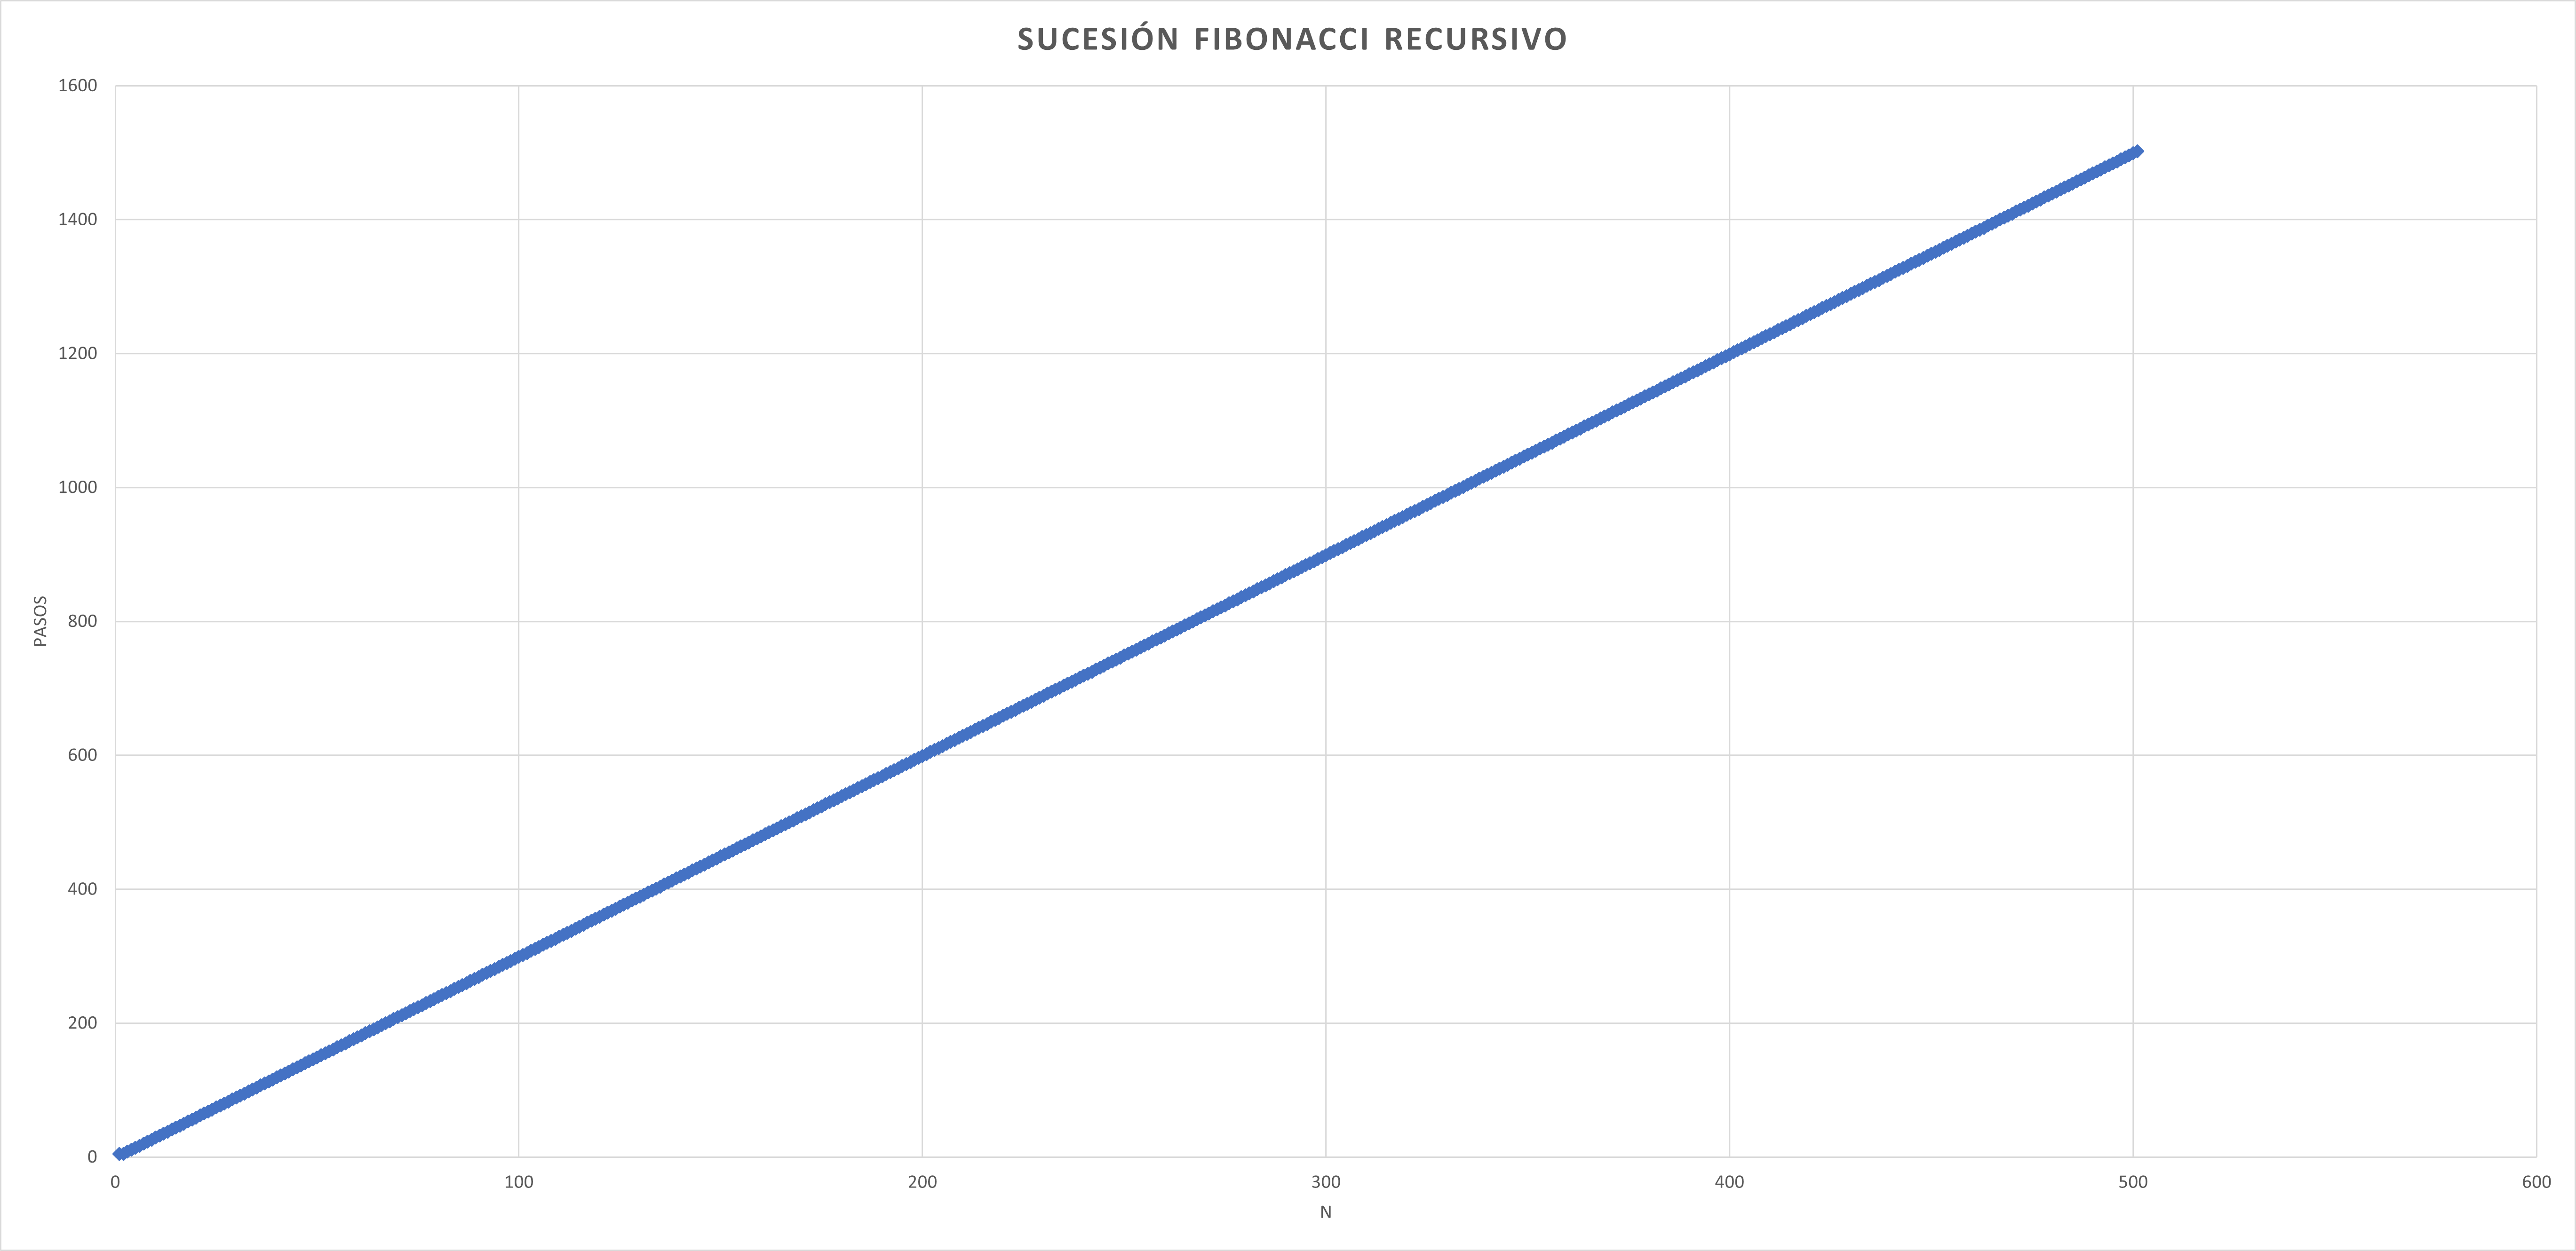
\includegraphics[width=1 \textwidth]{Images/posteriori_recursivo.png}  
            \caption{Análisis a Posteriori: Fibonacci Recursivo}
            \label{fig:recursivo_f}
        \end{figure}

\newpage
    \section{Algoritmo 3: Encontrar Numero Perfecto}
        El algoritmo codificado en \textit{Python} fue testeado en un entorno virtual de Linux en donde el algoritmo, en base a un numero como parametro de la funcion, pudo verificar si se trataba de un numero perfecto o no.
    
    \subsection{Análisis a Priori}
        En el análisis a priori del algoritmo para encontrar un número perfecto concluyó que el algoritmo presenta una complejidad lineal, esto debido a que el for ciclico solamente realiza una operación y acumula una sola variable en cada iteración. El análisis fue realizado sobre el código fuente, se puede observar en la figura \ref{fig:perfecto_priori}.
        \begin{figure}[htp!]
            \centering
            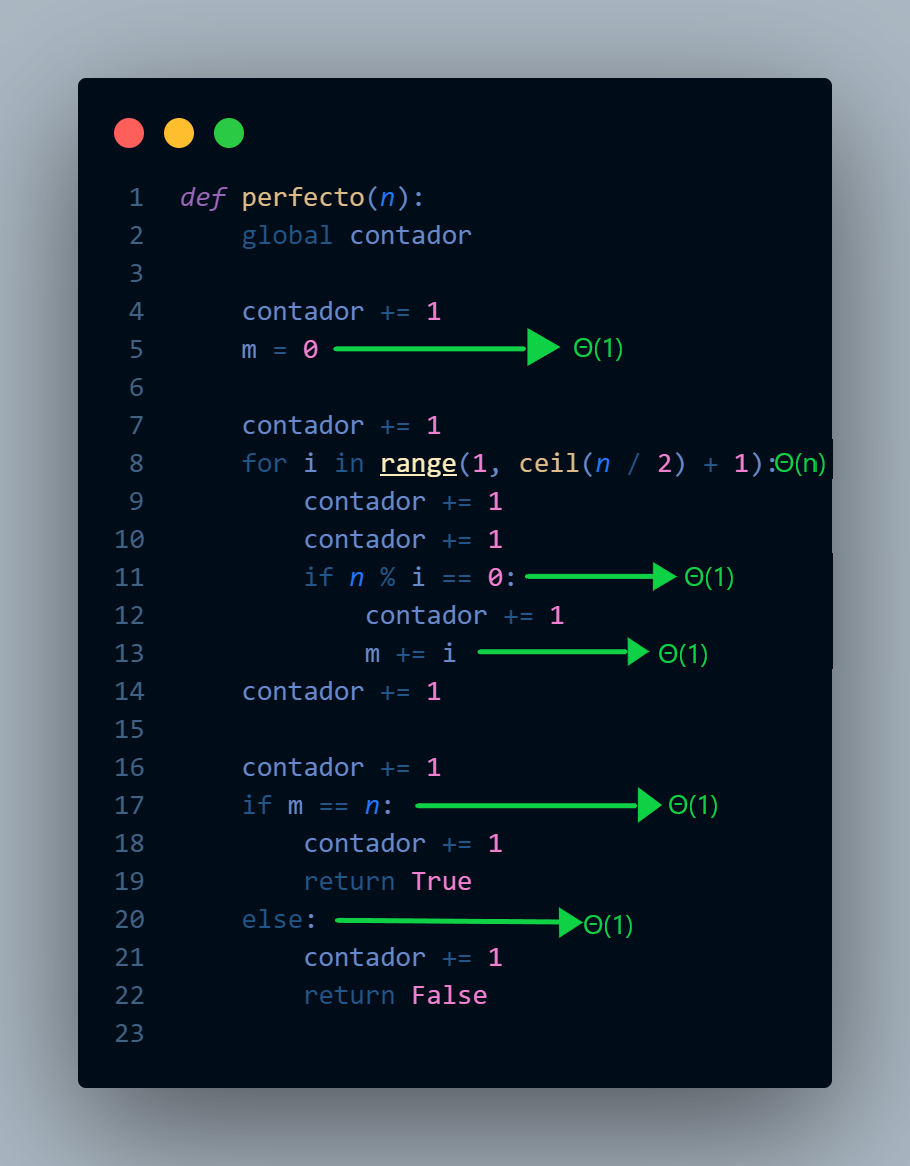
\includegraphics[width=0.6 \textwidth]{Images/priori_perfecto.png}
            \caption{Análisis a Priori: Encontrar Perfecto}
            \label{fig:perfecto_priori}
        \end{figure}
    
    \newpage   
    \subsection{Analisis a Posteriori}
        Con los resultados, se observa que el algoritmo requiere más pasos conforme el número de entradas incrementa. En la figura \ref{fig:perfecto_post_1} tal podemos observar que esto se cumple dentro de la función.
        
        \begin{figure}[htp!]
            \centering
            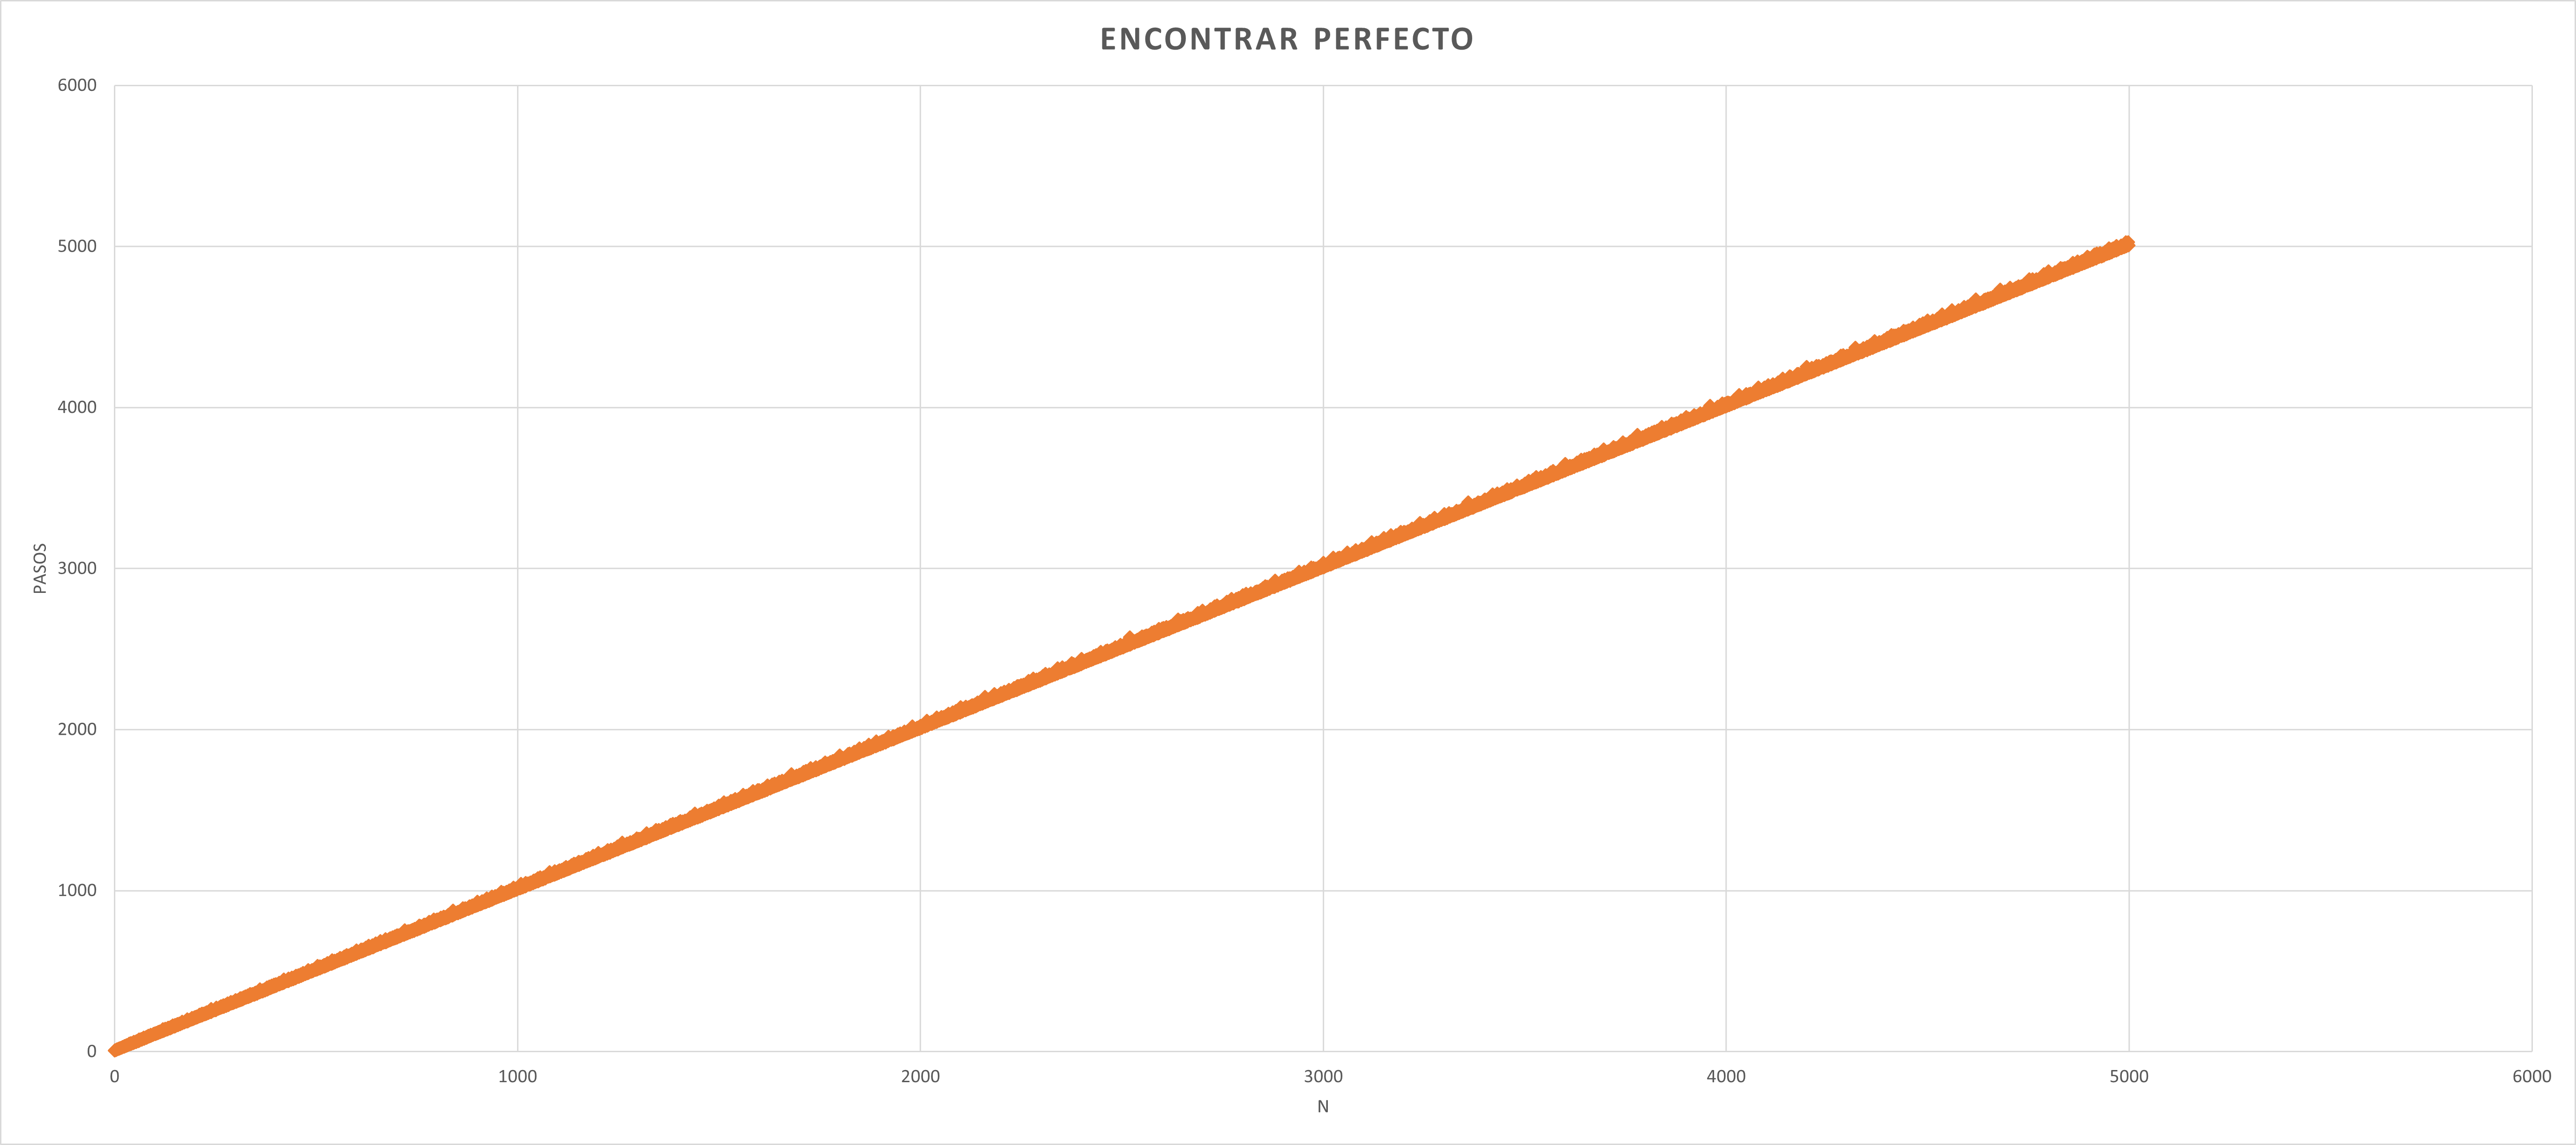
\includegraphics[width=0.8 \textwidth]{Images/posteriori_perfecto.png}
            \caption{Análisis a Posteriori: Encontrar Perfecto}
            \label{fig:perfecto_post_1}
        \end{figure}

\newpage
    \section{Algoritmo 4: Mostrar Numeros Perfectos}
        El algoritmo codificado en \textit{Python} fue testeado en un entorno virtual de Linux en donde el algoritmo verifica junto con la función \textit{Perfecto()} que un número sea perfecto para después mostrarlo en pantalla. Esta función numera los números perfectos. 
        
    \subsection{Analisis a Posteriori}
        El algoritmo analizado a posteriori dio como resultado que existen 6 números perfectos en un conjunto de 5 mil números. En la figura \ref{fig:perfecto_post_2} se observa que se ocuparon más de 350 millones de pasos para poder encontrar el sexto número perfecto. 
        
        \begin{figure}[htp!]
            \centering
            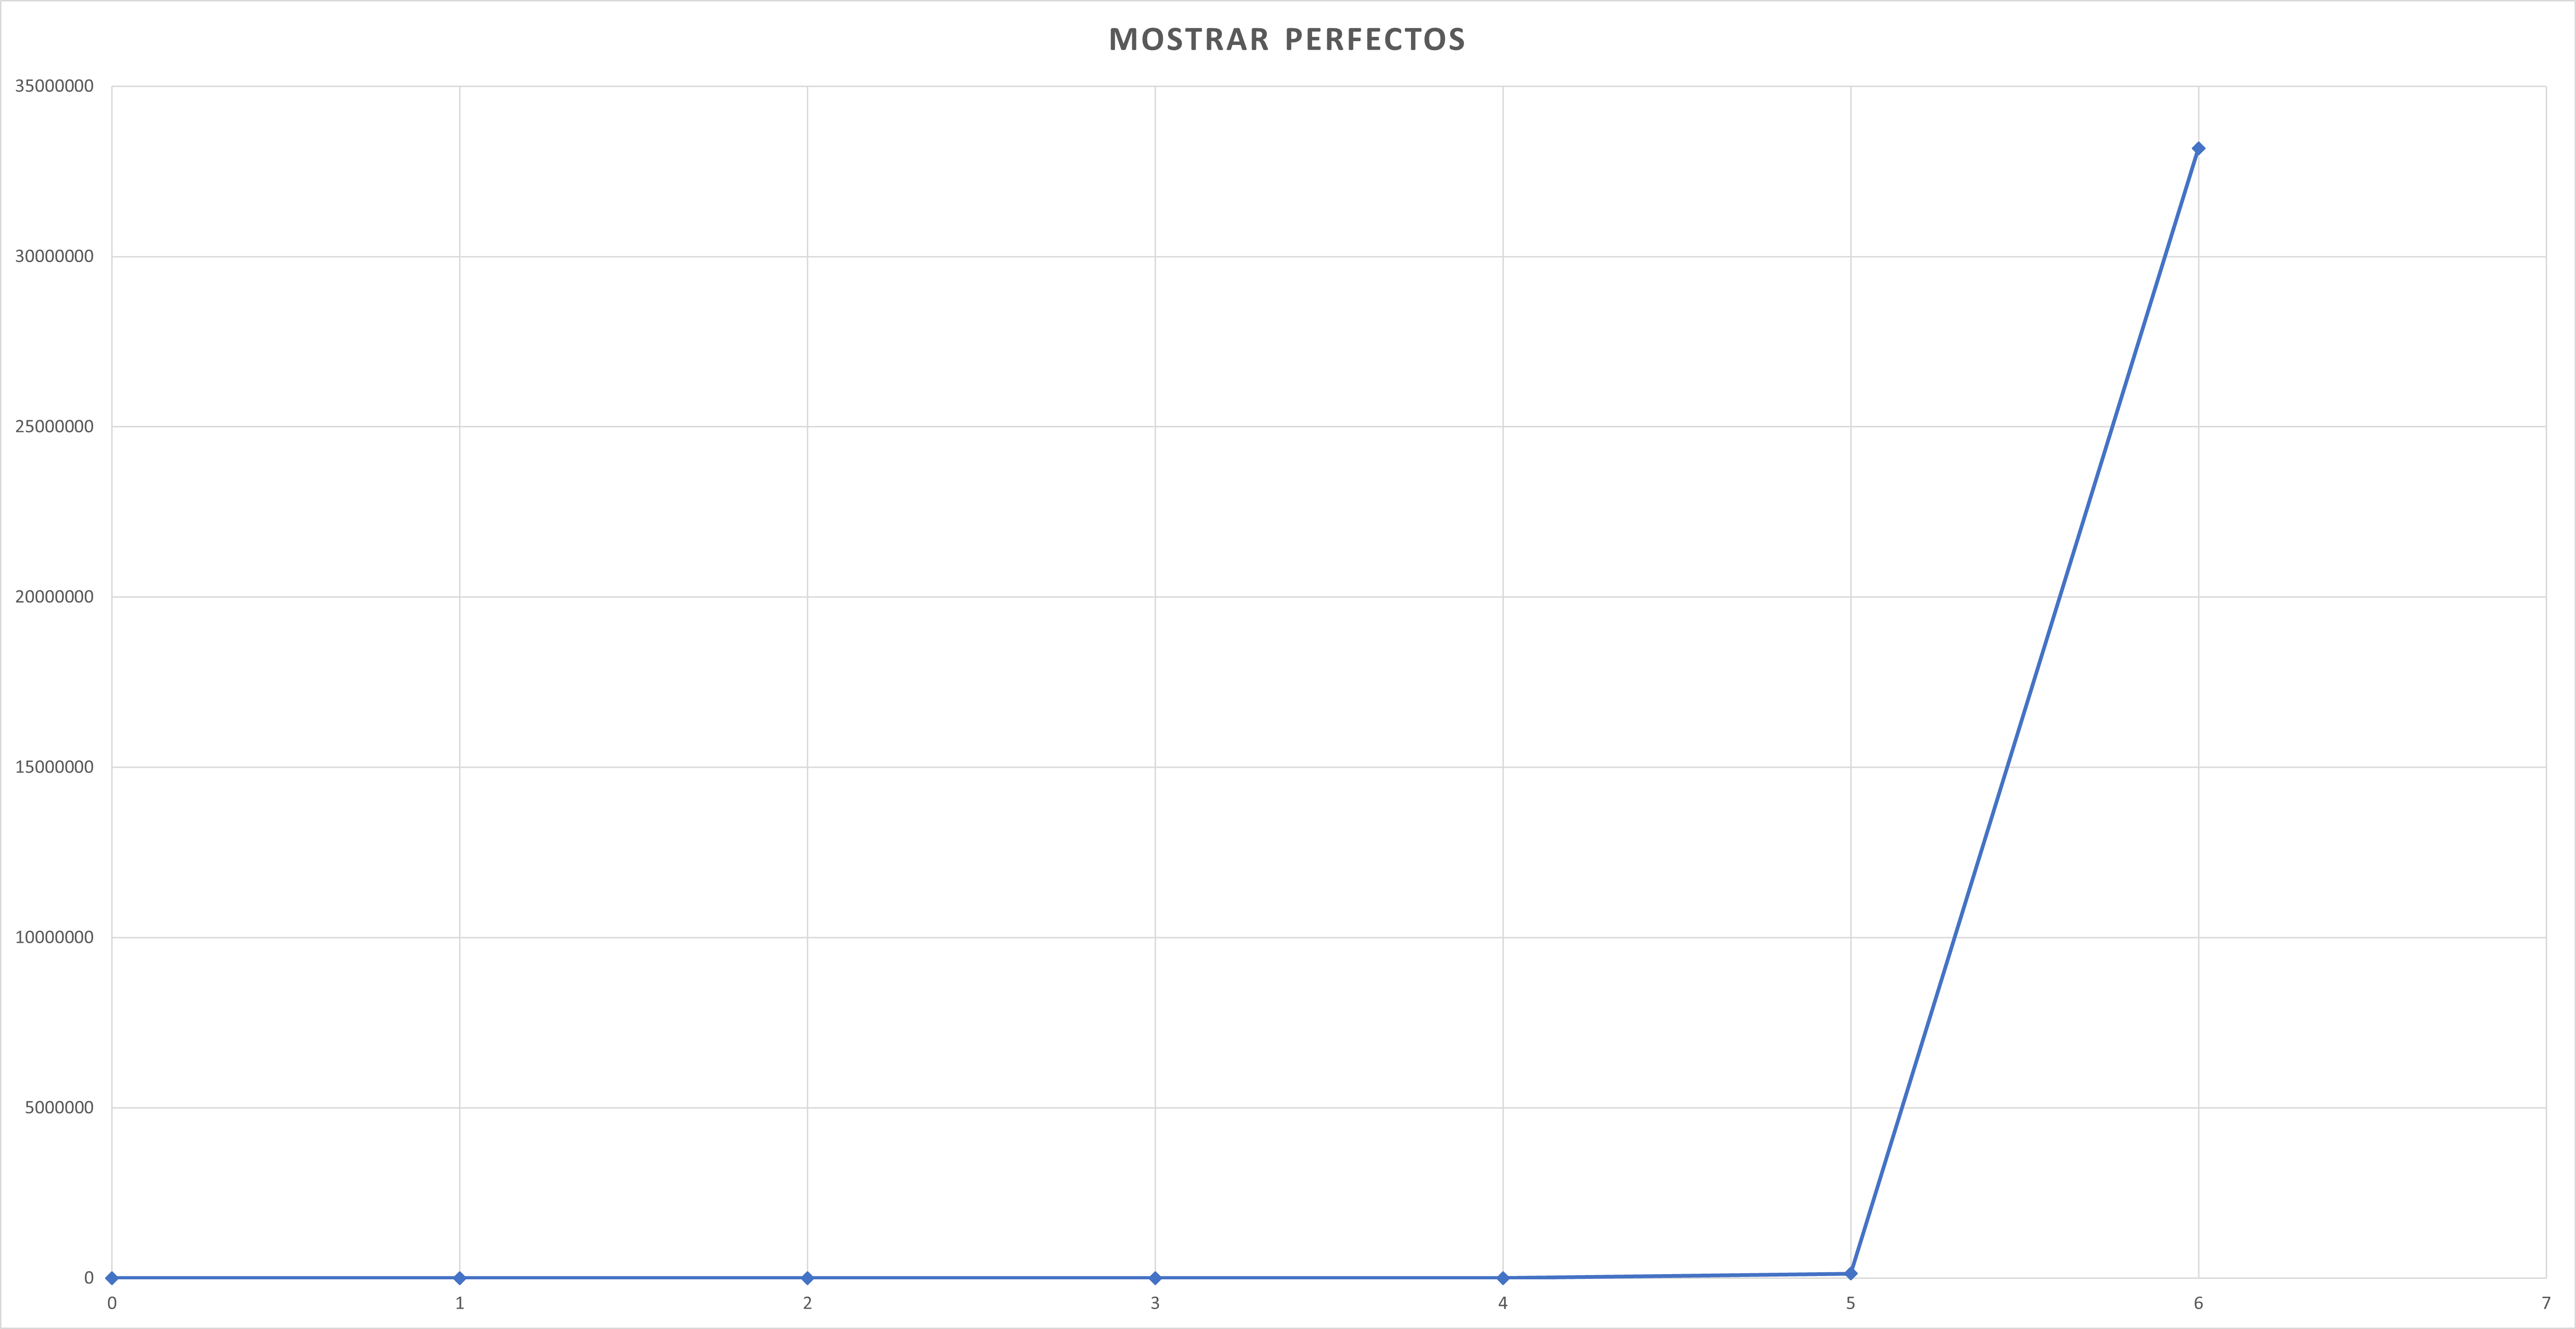
\includegraphics[width=0.8 \textwidth]{Images/posteriori_perfecto_m.png}
            \caption{Análisis a Posteriori: Mostrar Perfecto}
            \label{fig:perfecto_post_2}
        \end{figure}
        
        
    
